\documentclass[12pt]{article}

%%%%%%%%%%%%%%%%%%%%%%%%%%%%%%%%%%%%%%%%%%%%%%%%%%%%%%%%%%%%%%%%%%%%%%%%%%%%%%%%%%%%%%%%%%%%%%%%%%%%
% Math
\usepackage{fancyhdr} 
\usepackage{amsfonts}
\usepackage{amsmath}
\usepackage{amssymb}
\usepackage{amsthm}
\usepackage{enumitem}
%\usepackage{dsfont}

%%%%%%%%%%%%%%%%%%%%%%%%%%%%%%%%%%%%%%%%%%%%%%%%%%%%%%%%%%%%%%%%%%%%%%%%%%%%%%%%%%%%%%%%%%%%%%%%%%%%
% Macros
\usepackage{calc}

%%%%%%%%%%%%%%%%%%%%%%%%%%%%%%%%%%%%%%%%%%%%%%%%%%%%%%%%%%%%%%%%%%%%%%%%%%%%%%%%%%%%%%%%%%%%%%%%%%%%
% Commands and Custom Variables	
\newcommand{\problem}[1]{\hspace{-4 ex} \large \textbf{Problem #1} }
\let\oldemptyset\emptyset
\let\emptyset\varnothing
\newcommand{\norm}[1]{\left\lVert#1\right\rVert}
\newcommand{\sint}{\text{s}\kern-5pt\int}
\newcommand{\powerset}{\mathcal{P}}
\renewenvironment{proof}{\hspace{-4 ex} \emph{Proof}:}{\qed}
\newcommand{\RR}{\mathbb{R}}
\newcommand{\NN}{\mathbb{N}}
\newcommand{\QQ}{\mathbb{Q}}
\newcommand{\ZZ}{\mathbb{Z}}
\newcommand{\CC}{\mathbb{C}}
\renewcommand{\Re}{\operatorname{Re}}
\renewcommand{\Im}{\operatorname{Im}}

\newcommand{\solution}{\vspace{2 ex} \hspace{-5 ex} \emph{Solution.} }


%%%%%%%%%%%%%%%%%%%%%%%%%%%%%%%%%%%%%%%%%%%%%%%%%%%%%%%%%%%%%%%%%%%%%%%%%%%%%%%%%%%%%%%%%%%%%%%%%%%%
%page
\usepackage[margin=1in]{geometry}
\usepackage{setspace}
%\doublespacing
\allowdisplaybreaks
\pagestyle{fancy}
\fancyhf{}
\rhead{Malmuth \& Shaw \space \thepage}
\setlength\parindent{0pt}

%%%%%%%%%%%%%%%%%%%%%%%%%%%%%%%%%%%%%%%%%%%%%%%%%%%%%%%%%%%%%%%%%%%%%%%%%%%%%%%%%%%%%%%%%%%%%%%%%%%%
%Code
\usepackage{listings}
\usepackage{courier}
\lstset{
	language=Python,
	showstringspaces=false,
	formfeed=newpage,
	tabsize=4,
	commentstyle=\itshape,
	basicstyle=\ttfamily,
}

%%%%%%%%%%%%%%%%%%%%%%%%%%%%%%%%%%%%%%%%%%%%%%%%%%%%%%%%%%%%%%%%%%%%%%%%%%%%%%%%%%%%%%%%%%%%%%%%%%%%
%Images
\usepackage{graphicx}
\graphicspath{ {images/} }
\usepackage{float}

%tikz
\usepackage[utf8]{inputenc}
\usepackage{pgfplots}
\usepgfplotslibrary{groupplots}

%%%%%%%%%%%%%%%%%%%%%%%%%%%%%%%%%%%%%%%%%%%%%%%%%%%%%%%%%%%%%%%%%%%%%%%%%%%%%%%%%%%%%%%%%%%%%%%%%%%%
%Hyperlinks
%\usepackage{hyperref}
%\hypersetup{
%	colorlinks=true,
%	linkcolor=blue,
%	filecolor=magenta,      
%	urlcolor=cyan,
%}

\begin{document}
	\thispagestyle{empty}
	
	\begin{flushright}
		Daniel Malmuth \& Sage Shaw \\
		m566 - Spring 2018 \\
		\today
	\end{flushright}
	
{\large \textbf{HW - Chapter 9}}\bigbreak

\problem{8} In considering the non-linear partial differential equation
$$
-\left( \frac{\partial^2 u }{\partial x^2} + \frac{\partial^2 u }{\partial y^2} \right) - e^u = 0
$$
we seek solutions by approximating the laplacian with the 5-point finite difference operator on a mesh of step size $h=1/(N+1)=2^{-7}$, and then solving the non-linear system of equations using Newton's Method for systems of equations. After applying our FD approximation we have the following formulae
$$
4u_{i,j} - u_{i-1,j} - u_{i+1,j} - u_{i,j-1} - u_{i,j+1} - h^2e^{u_{i,j}} = 0
$$
for $1 \leq i,j \leq N+1$. Note that this problem is with the Dirichlet boundary conditions so $0 = u_{0,j} = u_{i,0} =  u_{N+1,j} = u_{i,N+1}$ for all points along the boundary. These systems can be represented using the matrix equation
$$
A\vec{u} - h^2e^{\vec{u}} = 0
$$
where $e^{\vec{u}}$ is element-wise exponentiation. The Jacobian of this is simply
$$
J(\vec{u}) = A - h^2 \text{diag}(e^{\vec{u}})
$$
where $\text{diag}(\vec{x})$ is a square matrix with $\vec{x}$ on the main diagonal and zeros elsewhere. Python code for the implementation can be found in the appendix. \bigbreak

The solution can be seen in figure (\ref{p8}). The blue values represent $0$ as on the boundary and the maximum value of the solution is roughly $0.0780975$ near the center of the domain. The requested norms are given below. Newton's method required only 2 iterations to converge. \\

We were unable to find a second solution to this PDE. Using either formula for the initial vector given by $u(x,y) = ax(1-x)(1-y)$ or $u(x,y) = axy(1-x)(1-y)$ and trying several thousand values of $a$ ranging from -2000 to 2000, all initial vectors either converged to the same solution or failed to converge.

\begin{align*}
\frac{\norm{\vec{u}}_2}{\sqrt{n}} &= 0.0438569 \\
\norm{\text{exp}(\vec{u})}_\infty &= 1.08123
\end{align*}

\begin{figure}[H]
	\caption{Colormap of the solution over the unit square.}
	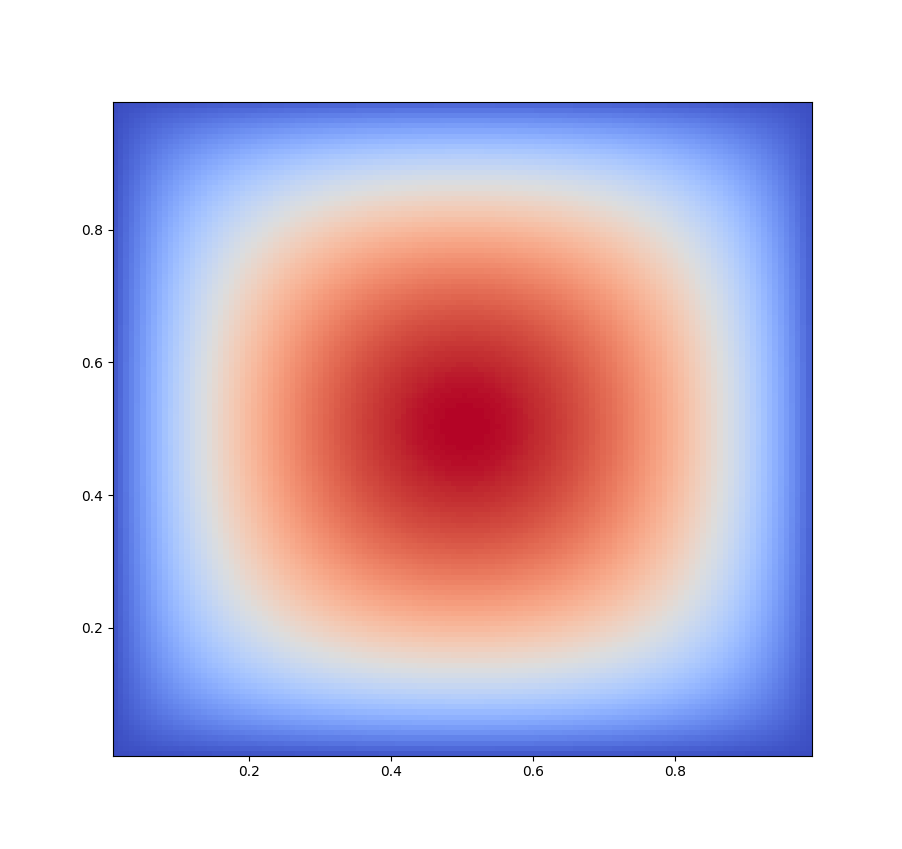
\includegraphics[width=1\textwidth]{hwch9_p8_figure_1}
	\label{p8}
	\centering
\end{figure}

\bigbreak
%%%%%%%%%%%%%%%%%%%%%%%%%%%%%%%%%%%%%%%%%%%%%%%%%%%%%%%%%%%%%%%%%%%%%%%%%%%%%%%%%%%%%%%%%%%%%%%%%%%%

\problem{9} We chose Conjugate Gradient as our Krylov subspace method. The implementation can be found in the appendix. The summary from running the method is as follows
\begin{lstlisting}
n = 16129
CG iterations: 636
CG iterations: 12686
CG iterations: 10589
CG iterations: 13425
Newton's Method iterations: 5
\end{lstlisting}
For a direct solve we expect roughly $\mathcal{O}(n^3)$ for each iteration of Newton's method. However, the matrices we're solving here are sparse, and in particular $N$-banded so we expect an iteration to be roughly on the order of $\mathcal{O}(Nn^2) = \mathcal{O}(n^{2.5})$ depending on the direct solve method.  \\

An iteration of Conjugate Gradient is about as expensive as a matrix vector multiplication in general, but since the matrix is quite sparse this cost is roughly $\mathcal{O}(n)$. In theory Conjugate Gradient takes at most $n$ iterations to converge, but since we are only searching for approximate solutions, it will take fewer. This puts one iteration of the Inexact Newton's method at less that $\mathcal{O}(n^2)$. In order to be bested by the Exact Newton's method, the Inexact Newton's method using CG would need $\mathcal{O}(\sqrt{n})$, far more than the few iterations it required to converge. \\

We conclude that for this problem (and others that are similarly sparse) the Inexact Newton's method with Conjugate Gradient as the iterative step is faster by at least $\mathcal{O}(n)$ in theory.

\bigbreak
%%%%%%%%%%%%%%%%%%%%%%%%%%%%%%%%%%%%%%%%%%%%%%%%%%%%%%%%%%%%%%%%%%%%%%%%%%%%%%%%%%%%%%%%%%%%%%%%%%%%

{\hspace{-4 ex} \huge \textbf{Appendix - Code listings}}\bigbreak
\problem{8 - Code}
\begin{lstlisting}
#sparse solver
N = 2**7-1
n = N**2
h = 1/(N+1)

a = .1
iter_max = 100
tol = 10**-6


J = np.diag([4]*N) + np.diag([-1]*(N-1),k=-1) + np.diag([-1]*(N-1),k=1)
K = np.diag([-1]*N)
shape_matrix = np.diag([1]*(N-1),k=-1) + np.diag([1]*(N-1),k=1)
A = sparse.lil_matrix(np.kron(shape_matrix,K) + np.kron(np.eye(N),J))

# generate initial u
X = np.linspace(h,1-h,N)
u = np.array([ a*x*(1-x)*(1-y) for x in X for y in X]).reshape((n,1))

#u = np.ones((n,1))
Jac = A - sparse.diags(h**2*np.exp(u).ravel())
u_new = u + spsolve(Jac, h**2*np.exp(u) - A.dot(u)).reshape((n,1))
for iteration in range(1,iter_max+1):
	if la.norm(u_new-u) < tol*n:
		break
	u = u_new
	Jac = A - sparse.diags(h**2*np.exp(u).ravel())
	u_new = u + spsolve(Jac, h**2*np.exp(u) - A.dot(u)).reshape((n,1))

u = u_new

print(iteration)
X, Y = np.meshgrid(np.linspace(h,1-h,N),np.linspace(h,1-h,N))
U = u.reshape((N,N))
plt.pcolormesh(X,Y,U, cmap=cm.coolwarm)
\end{lstlisting}

Code searching for second solutions to the PDE
\begin{lstlisting}
def sparse_solver_CG(N, a, tol=10**-10):
	n = N**2
	h = 1/(N+1)
	
	iter_max = 10**3
	#tol = 10**-6
	
	cg_iter = 10**10
	cg_tol = 10**-2
	
	
	J = np.diag([4]*N) + np.diag([-1]*(N-1),k=-1) + np.diag([-1]*(N-1),k=1)
	K = np.diag([-1]*N)
	shape_matrix = np.diag([1]*(N-1),k=-1) + np.diag([1]*(N-1),k=1)
	A = sparse.lil_matrix(np.kron(shape_matrix,K) + np.kron(np.eye(N),J))
	
	# generate initial u
	X = np.linspace(h,1-h,N)
	u = np.array([ a*x*y*(1-x)*(1-y) for x in X for y in X]).reshape((n,1))
	
	#u = np.ones((n,1))
	Jac = A - sparse.diags(h**2*np.exp(u).ravel())
	u_new = u + conjugate_gradient(Jac, h**2*np.exp(u) - A.dot(u), u, tol=cg_tol, max_iter=cg_iter)[0].reshape((n,1))
	for iteration in range(1,iter_max+1):
		if la.norm(u_new-u) < tol*n:
			break
		u = u_new
		Jac = A - sparse.diags(h**2*np.exp(u).ravel())
		u_new = u + conjugate_gradient(Jac, h**2*np.exp(u) - A.dot(u), u, tol=cg_tol, max_iter=cg_iter)[0].reshape((n,1))
		assert u_new.shape==u.shape
	
	return u_new

N = 2**5-1
n = N**2

u = sparse_solver_CG(N,.1)
for a in np.linspace(-100,100,1000):
	u_0 = np.random.randn(n)
	u_new = sparse_solver_CG(N,a)
	print('a=%f, diff=%g' % (a,la.norm(u - u_new)) )
	if la.norm(u - u_new) > 10**-2:
		break

print(iteration)
X, Y = np.meshgrid(np.linspace(h,1-h,N),np.linspace(h,1-h,N))
U = u.reshape((N,N))
plt.pcolormesh(X,Y,U, cmap=cm.coolwarm)
U = u_new.reshape((N,N))
plt.pcolormesh(X,Y,U, cmap=cm.coolwarm)
\end{lstlisting}


\problem{9 - Code}
\begin{lstlisting}
def conjugate_gradient(A, b, x_0, tol=10**-2, max_iter=10**3):
	x = x_0
	r = b - A.dot(x)
	delta = np.dot(r.T,r)
	b_delta = np.dot(b.T,b)
	p = r
	for k in range(max_iter):
		if delta < b_delta * tol**2:
			break
		s = A.dot(p)
		alpha = delta/(np.dot(p.T,s))
		x_new = x + p*alpha
		r -= s*alpha
		delta_new = np.dot(r.T,r)
		p = r + p*delta_new/delta
		x, delta = x_new, delta_new
	return x, k

#sparse solver - CG
N = 2**7-1
n = N**2
h = 1/(N+1)
print('n = %d' % n)

a = .5
iter_max = 10**3
tol = 10**-10

cg_iter = 10**10
cg_tol = 10**-2


J = np.diag([4]*N) + np.diag([-1]*(N-1),k=-1) + np.diag([-1]*(N-1),k=1)
K = np.diag([-1]*N)
shape_matrix = np.diag([1]*(N-1),k=-1) + np.diag([1]*(N-1),k=1)
A = sparse.lil_matrix(np.kron(shape_matrix,K) + np.kron(np.eye(N),J))

# generate initial u
X = np.linspace(h,1-h,N)
u = np.array([ a*x*(1-x)*(1-y) for x in X for y in X]).reshape((n,1))

#u = np.ones((n,1))
Jac = A - sparse.diags(h**2*np.exp(u).ravel())
CG, k = conjugate_gradient(Jac, h**2*np.exp(u) - A.dot(u), u, tol=cg_tol, max_iter=cg_iter)
u_new = u + CG.reshape((n,1))
for iteration in range(1,iter_max+1):
	if la.norm(u_new-u) < tol*n:
		break
	u = u_new
	Jac = A - sparse.diags(h**2*np.exp(u).ravel())
	CG, k = conjugate_gradient(Jac, h**2*np.exp(u) - A.dot(u), u, tol=cg_tol, max_iter=cg_iter)
	print('CG iterations: %d' % k)
u_new = u + CG.reshape((n,1))
assert u_new.shape==u.shape

u = u_new

print("Newton's Method iterations: %d" %iteration)
X, Y = np.meshgrid(np.linspace(h,1-h,N),np.linspace(h,1-h,N))
U = u.reshape((N,N))
plt.pcolormesh(X,Y,U, cmap=cm.coolwarm)
\end{lstlisting}



\end{document}
